\documentclass[12pt]{article}
\usepackage{amsmath}
\usepackage{amsfonts}
\usepackage{geometry}
\usepackage{graphicx}
\usepackage{setspace}
\usepackage{parskip}
\usepackage{hyperref}
\usepackage{float}
\usepackage{booktabs}
\usepackage{glossaries}
\usepackage{subcaption} % in your preamble

% Image optimization settings
% Configure image compression for XeTeX
\setkeys{Gin}{draft=false}

\geometry{a4paper, margin=1in}
\setstretch{1.2}

\title{\Huge Autonomous Bitcoin Trading\\\vspace{1cm}\Large Documentation}
\author{
    \Large Gymnasium Thun\\
     26gs\\
    \vspace{1cm}
    \Large Submitted by:\\
    \vspace{0.5cm}
    \textbf{Juri Stoffers}\\
    \vspace{2cm}
    \Large Supervised by:\\
    \vspace{0.5cm}
    \textbf{Dr. Geoffrey Ostrin}
}
\date{\Large \today}

\begin{document}

% Title page
\pagenumbering{gobble}
\maketitle
\clearpage

% Abstract
\pagenumbering{roman}
\begin{abstract}
    This thesis investigates the development and implementation of an autonomous Bitcoin trading algorithm, addressing the challenges of human emotion and bias in cryptocurrency trading. 
    Starting from the observation that human emotion based decision making, disables traders to act on opportunity in the markets. 
    The research combines technical analysis with algorithmic trading, employing a quantitative methodology that includes data collection. Strategy development using Python, and testing strategies on historical price data. The implementation involves creating a custom backtesting framework, developing rule-based trading strategies, and deploying a live trading system on a Linux based server.

\end{abstract}
\clearpage

% Continue roman numbering from abstract
\section*{Foreword}
Everything started somwhere in early 2022 where I read "The Bitcoin Standard" by Saifedean Ammous. A book explaining why Bitcoin even exists and what problem it is trying to solve. I probably only understood 30\% of the book. These 30\% however were enough for me to to start researching Bitcoin and the underlying technology. I watched regular Crypto Market update videos. Then in Novber 2022 FTX experienced a bank run.
FTX was the second largest Crypto exchange. (A place to sell and buy various Crypto currencies). The problem was FTX didn't have the exchange funds to cover the withdrawals. This was a big problem because FTX was the second largest exchange. Bitcoin already was down bad from previous highs but this was the final nail in the coffin. Bitcoin was down 80\% from its all time high and went down to a price of 15'000 dollars per Bitcoin.
That was the first time I wanted to buy Bitcoin after watching it for about half a year. Luckily in 2022 buying Bitcoin even when you are below 18 was possible.
One thing led to another and I spend more and more time watching charts and losing my mind. I tried to trade profitable.
This sounds very simple but it seemed impossible. I prefered to code and build my own projects since that gave you a consitent flow of results. With trading you never have consisted results you can sit in front of charts for a few hours and not do anything or even lose money. That is why I think combining coding and trading is a good idea.

I had no idea what I was getting myself into and if I knew before I would probably have never started. I spend more time than I wanted and complety lost myself in the work. I totaly fogrot about the writting part and spend a lot of time just coding. This whole thing got way bigger than I initially thought but I'm proud to present what I got since it is a lot.





\clearpage

% Table of contents
\pagenumbering{roman}
\tableofcontents
\clearpage

% Start main content with arabic numbering
\pagenumbering{arabic}
\setcounter{page}{1}
\section{Introduction}
This thesis explores whether I can develop an autonomous trading algorithm that can generate me a consistent profit. To that end my thesis will cover the entire development cycle, from researching, backtesting strategies and live deployment execution with real money on Bitcoin evaluating the results in the end.


The strategy I will try to find should rely on  signals found by analysing historical Bitcoin data. The model will be tested on historical timeseries data.

The work is divided in three parts: Researching this can be done in multiple ways just by watching markets over longer time periods to get ideas, reading books about how other people were able to develope strategies and steal logic from them or just try to find something by yourself which can be implemented as a strategy.



The skills I need to complete this project are Luckily straight forward: Statistics, Programming and understanding how the market operates. I need to apply stasticial rules to check if my idea is worthless or has potential to make me a profit if i automate the execution process. Programming is just needed to make the process of testing or applyinng my ideas easy on large datasets since I have to test on timeseries up to 200'000 values. The algorithm will be written in Python and will run 24 hours a day seven days a week.





So I'm planning to end up with the following products at the end of this project:

\begin{itemize}
    \item Trading strategy
    \item Backtests results
    \item Research documentation
    \item Trading algorithm
    \item Live execution results
    \item Live Dashboard

\end{itemize}



\subsection{Trading strategy}
A trading strategy is a set of rules that are used to make a decision to buy or sell a asset. it can consistis out of systematic rules or purly based on discretionary rules.
Systematic rules are set for specific values to occure or a signals so for example if we move up 2\% in one day we buy x amount of Bitcoin. A discretionary rule is a rule that is based on a human's intuition or a feeling.

My algorithm trading strategy is clearly a systematic rule set since we can't automate discretionary rules.

\subsection{Backtesting Results}
To find an strategy we have to first test potential ideas on historical data after finding a potential strategy we can run backtests to see how it would have performed in historical environments




\subsection{Research documentation}
Throughout this research, I have documented the formulas used and detailed test results that were too extensive to include in the main thesis. This documentation serves as a companion piece, written to be understandable after reading the main thesis.


\subsection{Trading algorithm}
This will be in form of a github repository, github is a platform where you can share codebases and collaborate with other people.
It is the easiest way to share my code and make it available to other people. So in the Github repository I will share the codebase for my trading algorithm


\subsection{Live dashboard}
This will just be a website where you can see the live performance of the trading algorithm, the live signal calculations results and how my algorithm currently is positioned.



\newpage

\section{Theoretical Background}
\subsection{Digitalisation of Trading}
So when I am speaking of trading I mean the buying and selling of assets at an exchange. Before the digitalisation traders meet at exchanges to trade where they communicated with shouting and hand signals under each other to buy and sell assets from each other. The hand signals allowed the traders to communicate price, quantity and the type of order\footnote{An order is an instruction given by a trader to buy or sell a specific quantity of an asset, usually including details like the price and type of transaction (e.g., buy or sell).}
they wanted to set up.  All of this happened on so called "Trading Pits" which were located inside of exchanges.


In the late 20th century electronical systems gradualy replaced the communication used insde of the Trading Pit. Electronical systems brought a lot of advantages with them as orders could be executed faster, more cheaply and with improved record-keeping. Which opened the world of trading to a broader range of market participants. 
As electronical trading grew, the use of technical analysis grew too, in short TA, makes use of historical price data where patters can be watched and indicators to forcast price movementes.

Online brokerages enabled individuals to trade based on their own interoretation of TA without the need of giving out a form of physical trading signal.

With increased computing power, large institutions use trading algorithms which are automated programs that execute trades based on pre-set criteria, this could be various forms of technical analysis, price arbitrage\footnote{Arbitrage is a trading strategy that involves simultaneously buying and selling the same asset in different markets to profit from price differences. For example, if an asset is cheaper on one exchange than on another, a trader can buy it low and sell it high almost instantly.} or news events and a lot more.


Besides institutions, there are also individual traders who follow either a systematic/quantitative or discretionary approach. A systematic trader operates based on fixed criteria, while a discretionary trader relies on judgment, experience, and analysis. The key distinction is a discretionary trader cannot automate their trading strategy, whereas a systematic trader can, since they execute trades based on predefined entry conditions. These entry conditions often utilize technical indicators. For example, comparing two moving averages of different lengths. A simple formula like $MA_{short} > MA_{long}$ would be an example of such a fixed entry condition.

\newpage
\subsection{Efficient markets}
Making consistent profits in financial markets is difficult. Prices move in ways that often seem unpredictable, and most traders both discretionary and systematic struggle to gain a lasting edge. \footnote[1]{An edge is a consistent advantage over the market. It can be achieved through superior information, better analysis, or a unique trading approach.}One explination for this is the Efficient market hypothesis (EMH) which suggest that asset prices already reflect all available information, leaving little room for profitable oppertunities.


If the EMH were fully accurate in practice, then even the most advanced trading algorithms and best discretionary traders would not be able to consistently beat the market. \footnote[2]{Beating the market means achieving a higher ROI ("Return on Investment") than a certain benchmark. A common benchmark is the S\&P 500, which is an index including the 500 largest companies listed on U.S. stock exchanges. The S\&P 500 has had an average yearly return of about 10.33\% since 1957} Yet markets are not perfectly efficient, being heavily influenced by emotion, fear, and heard behaivour. Traders often fail to act on clear signals simply because it is psychologically hard to buy on a red day or sell while everybody is full of euphoria. 


To make things even better depending on where you trade market can change in efficient. But still some of the most valuable assets like stocks, gold and Bitcoin prices are a reflection of human emotion pricing in infromation. Especially now with Trump in office a lot of volatily came in with big oppertunities even on the higher time frame where the EMH is pretty accurate.  

Depending on the timeframe there are still a lot inefficient prices from which individuals can make a profit from. I will try to act on short term inefficient with my trading algorithm because I only have about one month for the live test and it would not make sense to run an algorithm which holds a trade over weeks and takes a trade every two months. In addition my initial idea when I started of with my matura thesis was already based on short term signals.§

It is possible to make a profit in the markets but it is not easy, not for everyone, and needs dedication. I am pretty sure I am able to make a profit. The question rather is if it is possible to do so in the limited time I have and at what scale.


\newpage

\subsection{Development of a Systematic Strategy}


The development of a systematic strategy typically follows several key steps:

\textbf{Idea Generation:}  
The process often begins with a hypothesis. For example, a trader might assume that when Bitcoin rises sharply within a short time, it tends to continue rising for a few more hours this would be a form of momentum. The idea must be simple enough to be coded, yet specific enough to be tested.

\textbf{Rule Definition:}  
Once the idea is clear, it is translated into precise entry and exit rules. For instance: "Buy Bitcoin if the 15-minute price increases by more than 1.5\% compared to the previous 60 minutes." Rules also include when to close a position, such as "Sell if the price drops 1\% below the entry."

\textbf{Backtesting:}  
The rules are then tested on historical data. This allows the developer to evaluate how the strategy would have performed in the past. Key performance metrics such as profit, win rate, drawdown, and Sharpe ratio are used to assess quality.

\textbf{Optimization and Robustness Testing:}  
After initial tests, parameters can be adjusted. For example, changing the percentage thresholds or time windows. However, this step must be handled with care — overfitting the strategy to past data may cause it to fail in real markets.

\textbf{Live Execution:}  
If the backtesting results are promising and the strategy appears robust, it can be deployed live. Execution is handled by a bot or script running on a server, which listens to market data and acts as soon as the conditions are met.

Throughout this process, the focus remains on consistency and measurability. Unlike human decision-making, a systematic strategy must behave identically entry and exit conditions. This makes it possible to evaluate, improve and automate trading in a transparent way.



\newpage
\section{Methodology}

\subsection{Project Overview}
The aim of this project was to design, test, and deploy a fully automated trading strategy for Bitcoin. The development process consisted of four main stages. First, historical price data was collected through a public exchange API and fetched in one minute intervals stored inside a database on a PaaS \footnote[1]{Stands for Platform as a service and it's a cloud computing model which gives developers a platform to host their applications so that they are globably accesable on the internet and run 24/7}. In the second stage, a simple rule-based strategy was defined based on technical indicators, with clearly specified entry and exit conditions. Next, the strategy was backtested on several months of historical data using a custom Python-based framework to evaluate its performance across different market conditions. Finally, if the results met predefined criteria (e.g. acceptable loses, stable returns), the strategy was deployed live on a cloud server that connects to the exchange and executes trades automatically in real time. Each stage of the process is documented in detail in the following sections.

\subsection{Data collection}




I chose to create my own dataset because it offers a key advantage: it allows me to experiment with ideas and patterns that are less likely to have been explored before. This increases the chance of discovering something new that might be missed when using more commonly available datasets.

In my dataset, I calculate the 1\%, 2.5\%, and 5\% delta of the order book. Additionally, I include the current Bitcoin price and the current timestamp. The program I wrote collects data by sending API requests \footnote[2]{API stands for Application Programming Interface. It is a tool that allows programs to request and receive specific data from external services in this case, used to fetch real-time Bitcoin price and orderbook data from the coinbase crypto exchange.} to the Coinbase Exchange API at one-minute intervals. It retrieves both the current Bitcoin price and a full snapshot of the order book at that moment. A complete snapshot is necessary to calculate order book deltas at different percentage depths accurately.

The script is hosted on my PaaS where my databse (Postgres) is also hosted where all the data is stored. It has been running 24/7 since March 11, 2025. 
\href{https://customchart-production.up.railway.app/#}{Live datamining progress}

The orderbook delta is calculated by summing the total value of bid orders $n\%$ below the current price ($P_t$) and subtracting the total value of ask orders that are $n\%$ above the current price ($P_t$).
\begin{equation*}
    \Delta_{OB} = \sum_{i=1}^{n} V_{bid_i} - \sum_{i=1}^{n} V_{ask_i}    
\end{equation*}




\newpage
\subsection{Designing and Developing Systems}


The most difficult part of developing a trading algorithm is finding a strategy that is actually worth integrating. As explained in the Efficient Markets section, it is in principle possible to find a strategy that generates profit. The problem is that finding a strategy which consistently makes money and outperforms the market is still extremely difficult.

Before I start searching, I need to define what I am searching for. To do this, I use the S.M.A.R.T. goal framework (Specific, Measurable, Attainable, Relevant, and Time-bound), as described in the book \href{https://www.amazon.com/Building-Winning-Algorithmic-Trading-Systems/dp/1118778987}{\textit{Building Winning Algorithmic Trading Systems}} by Kevin J. Davey.

\subsubsection*{Goals}
\begin{itemize}
    \item Two months allocated for finding a strategy
    \item Strategy operates on the Bitcoin/USD pair using \href{https://hyperfoundation.org/}{Hyperliquid}
    \item Target Sharpe ratio between 1 and 2 \footnote{The Sharpe ratio is a measure of risk-adjusted return. It compares the average return of a strategy to its volatility. A higher Sharpe ratio indicates a better balance between risk and return. A Sharpe ratio between 1 and 2 is considered decent in most financial contexts.}
    \item Approximately 20 trades per month
    \item No strict requirement to outperform the market; focus is on stability and consistency
\end{itemize}



%Starting of with searching for a potential strategy I already had a few ideas coming from discretionary trading approaches where I saw a potential to implement as a systemmatic set of rules. Just by reading tweets, watching crypto charts, and by playing with platforms offering various kinds of indicators. %One of the most significant advantages of crypto markets is the accessibility and granularity of trading data. Most major exchanges offer free public APIs that provide real-time and historical price data, often down to the minute or even second. This includes not only price and volume, but also open interest, funding rates, and even aggregated order book data in some cases. In contrast, similar datasets for traditional assets (e.g., stocks or futures) are often locked behind expensive data vendors or limited in granularity. The open nature of crypto data allows independent developers and researchers to prototype, test, and iterate much more rapidly — making it an ideal environment for building and evaluating automated strategies.
The area where I saw the most potential was the order book delta. My hypothesis was that, since it directly reflects the relationship between buyers and sellers at specific price levels, it could serve as the basis for a statistical signal. By running volatility and directional bias tests under various order book delta conditions, I aimed to identify patterns that might be predictive of short-term price movements.




% Smart strategy explination  why a goal is neede
% from where did I take inspiration 
% book I read
% testing testing and more testing
% where could I have done better
% how do the results macht with the live test
% Premutation tests and strategy development 


\newpage

\subsection{Searching/Backtesting}
As stated in my hypothesis: I think that the orderbook delta directly reflects the relationship between buyers and sellers at specific price levels. A strategy based on a negative order positive orderbook delta would not include enough context.

\begin{figure}[h]
    \centering
    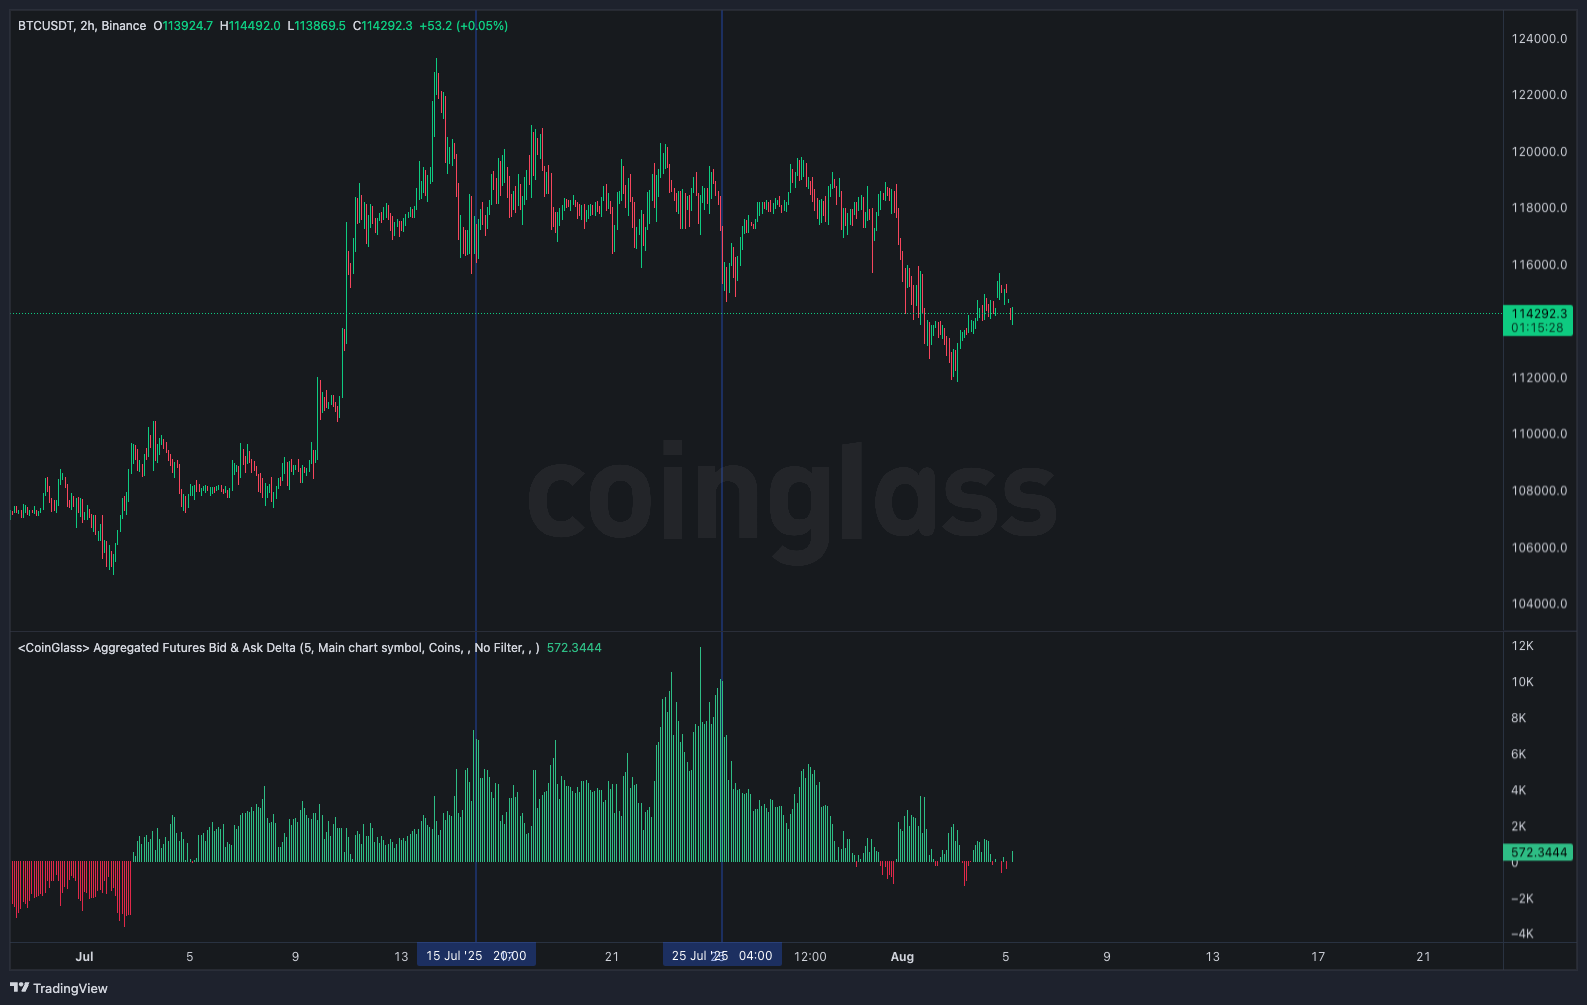
\includegraphics[width=0.95\textwidth]{imgs/showcase_chart.png}
    \caption{Orderbook delta visualization showing price action (top) and corresponding delta values (bottom)}
    \label{fig:orderbook_delta}
\end{figure}

As shown in Figure \ref{fig:orderbook_delta}, the orderbook delta provides valuable insights at extreme values. The chart displays two key components:
\begin{itemize}
    \item The price action (top chart) shows the actual Bitcoin price movements
    \item The orderbook delta (bottom chart) represents the imbalance between buy and sell orders
\end{itemize}

A high orderbook delta value indicates substantial buy orders below the current price. This creates a strong support level, as sellers would need significant pressure to break through these orders. Even if sellers manage to push through, these accumulated buy orders often create buying pressure that can lead to price support or potential rebounds.

This relationship between orderbook delta and price action is particularly useful when:
\begin{itemize}
    \item The delta reaches extreme values, indicating significant order imbalance
    \item There's a clear divergence between price action and orderbook delta
    \item Multiple timeframe analysis shows consistent patterns
\end{itemize}




\newpage
\textbf{Example:}

\begin{verbatim}
    #Example for entry signals in the code
    outlier_mask = (df['trend'] == 'uptrend') & (df['is_outlier'] == 1) 
\end{verbatim}

Then I test the strategy on one month of data to evaluate whether it shows any potential. I consider a strategy to have potential if it is around break-even \footnote{Break-even is the point where the total profit equals the total loss. In other words, it's the point where the strategy neither makes nor loses money.} or slightly profitable and achieves a Sharpe ratio between 1 and 2.

\textbf{Results:}

\begin{figure}[H]
    \centering
    \begin{subfigure}[b]{0.48\textwidth}
        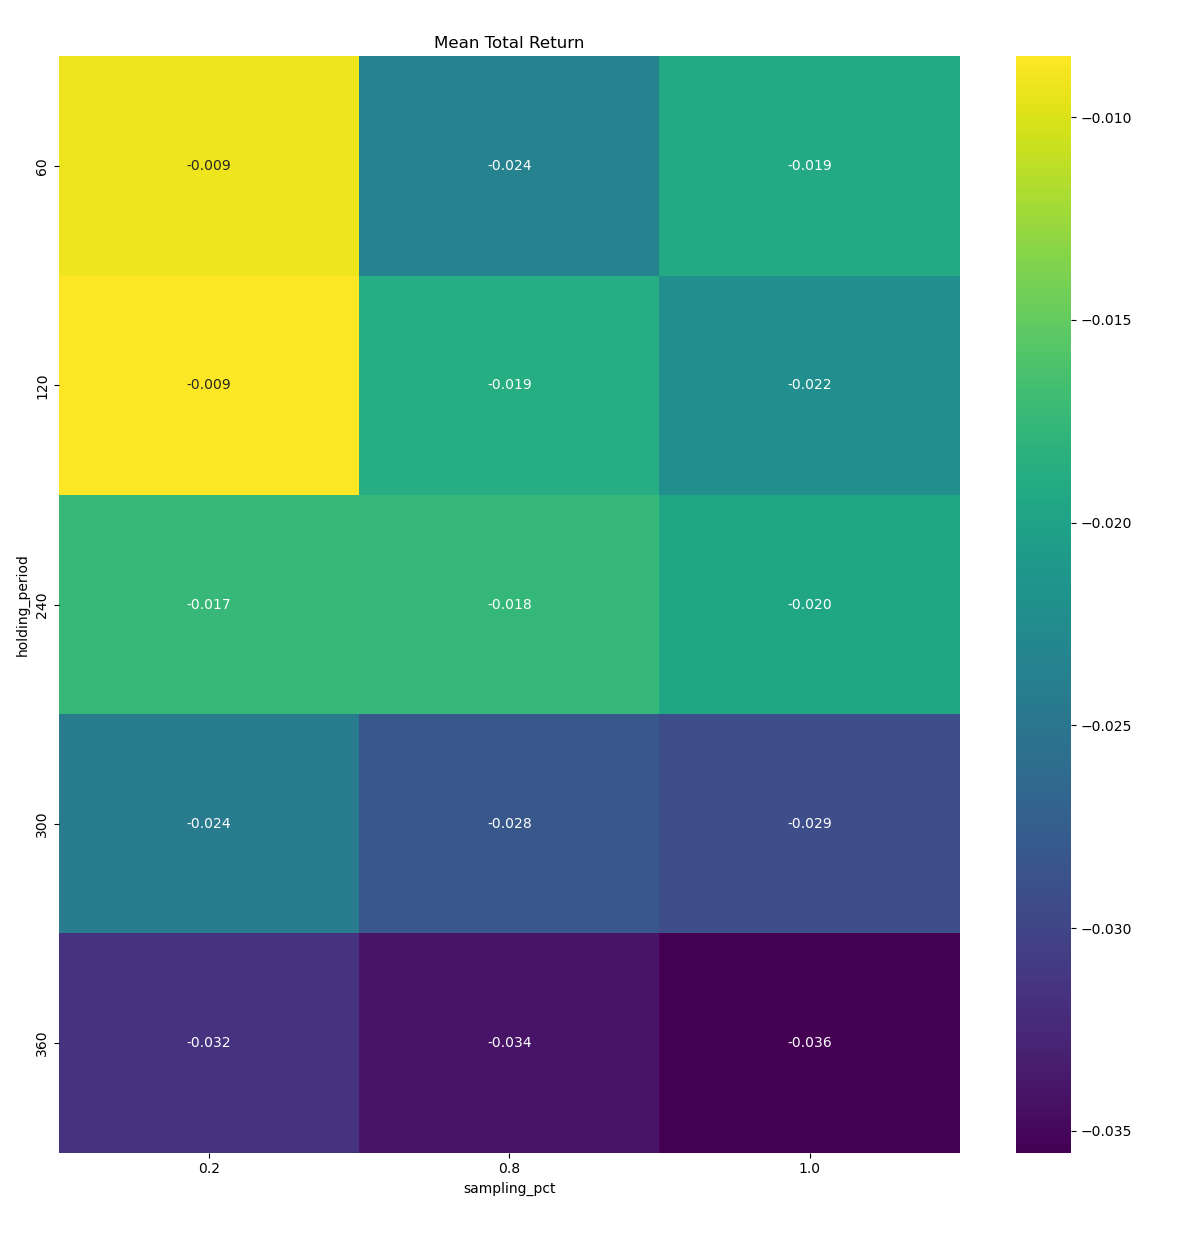
\includegraphics[width=\textwidth,height=0.3\textheight,keepaspectratio]{imgs/example_backtest_for_thesis.png}
        \caption{Bullish outliers}
        \label{fig:bullish_outliers}
    \end{subfigure}
    \hfill
    \begin{subfigure}[b]{0.48\textwidth}
        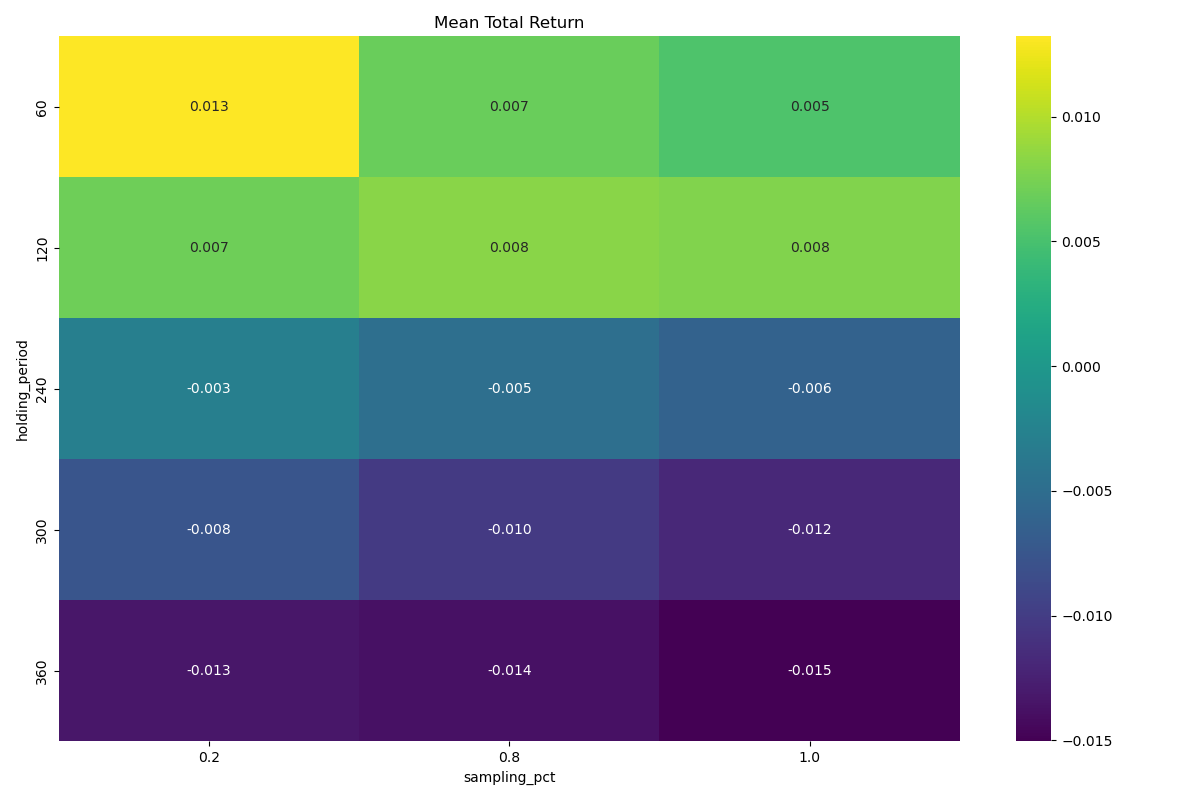
\includegraphics[width=\textwidth,height=0.3\textheight,keepaspectratio]{imgs/example_for_thesis_v2.png}
        \caption{Bullish outliers uptrend}
        \label{fig:bullish_outliers_uptrend}
    \end{subfigure}
    \caption{Just two examples of the backtest results}
    \label{fig:bullish_outliers_comparison}
\end{figure}

On the $X$ axis you can see the sample size and on the $Y$ axis you can see the average return over he different test runs.



\newpage
\section{Idea collection}
\begin{itemize}
    \item Trend = $\text{Uptrend if } \frac{d}{dt}\text{MA} > 0$
\end{itemize}


\newpage
\subsection{Related Work}
Discussion of related work.


\newpage
\section{Methodology}
Your methodology description.



\newpage

\end{document}

